\chapter{Literature Review}\label{cha:literature}

\section{State of the Art}\label{sec:state}

    \subsection{ROS on Web}\label{sub:ros_on_web}

        \begin{figure}[htbp]
            \centering
            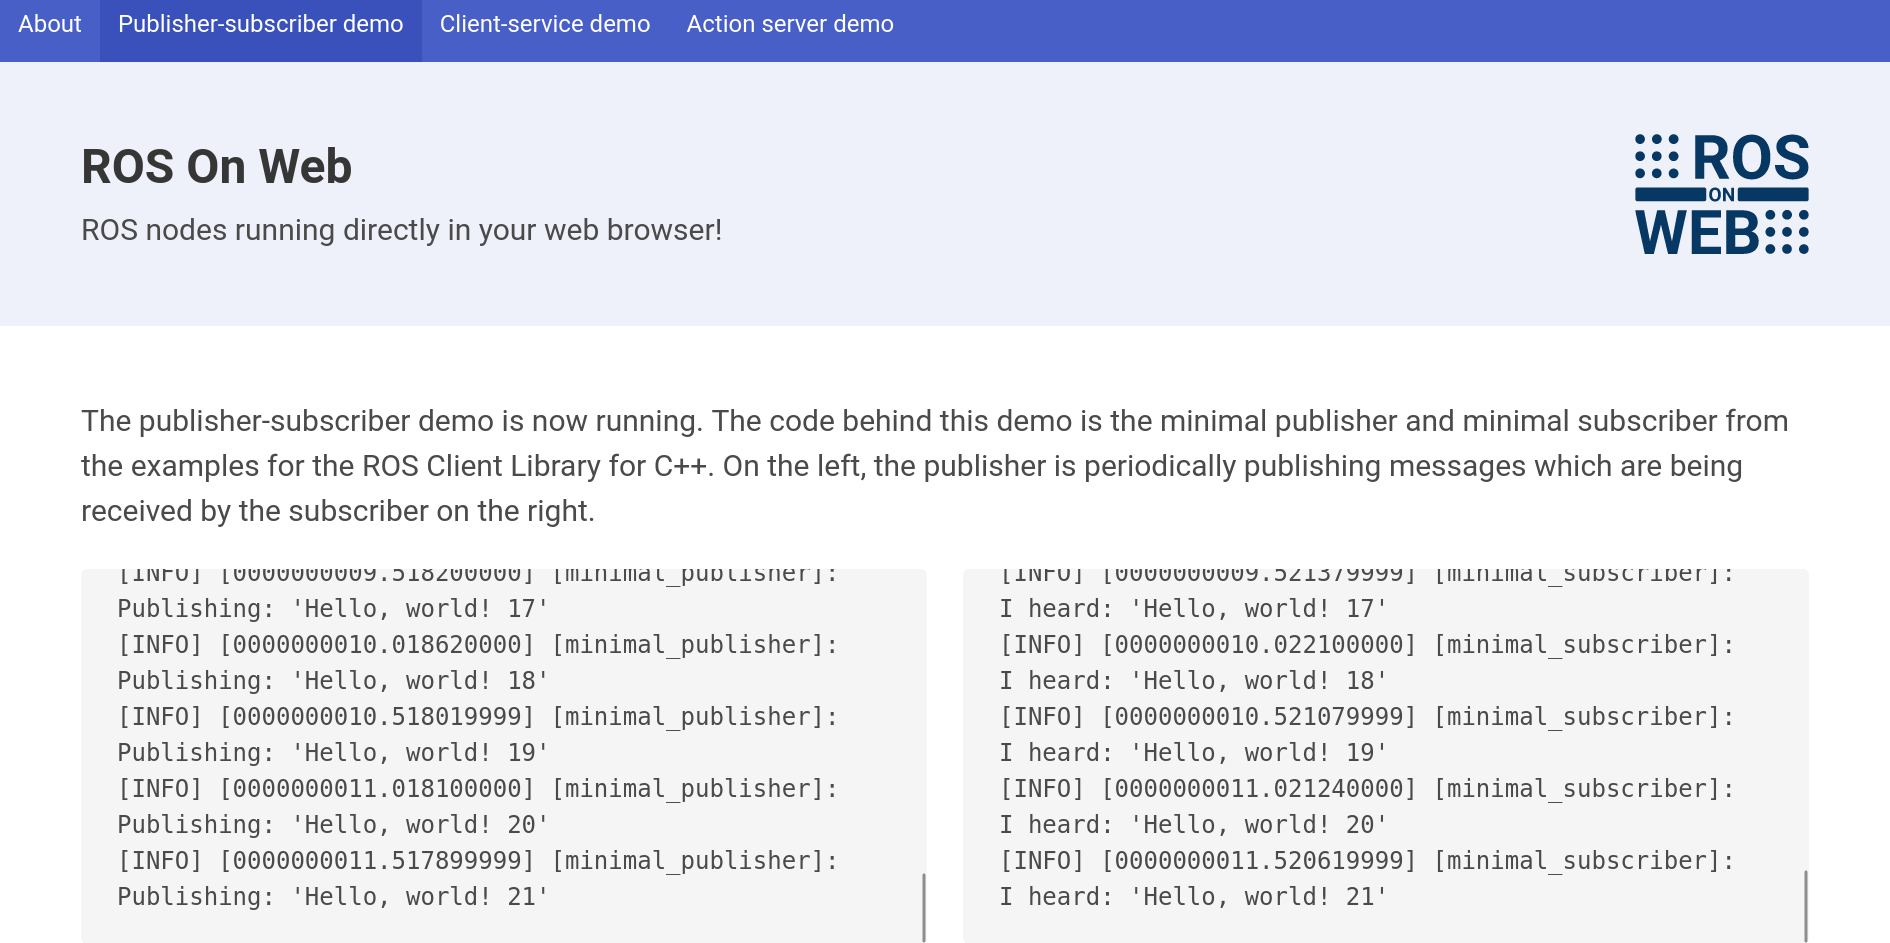
\includegraphics[width=\textwidth]{01_rosOnWeb.png}
            \caption{\textit{ROS on Web} publisher and subscriber demo}
        \end{figure}

        Advantages and disadvantages

        Not open source

        ROS1 or ROS2


\section{Relevant Works}

    \subsection{ROSbridge}

    \subsection{ROS Control Center}

    \subsection{ROSboard}

    \subsection{ROSlink}

    \subsection{Foxglove Studio}
        % https://foxglove.dev/blog/publishing-and-visualizing-ros2-transforms

        \begin{figure}[htbp]
            \centering
            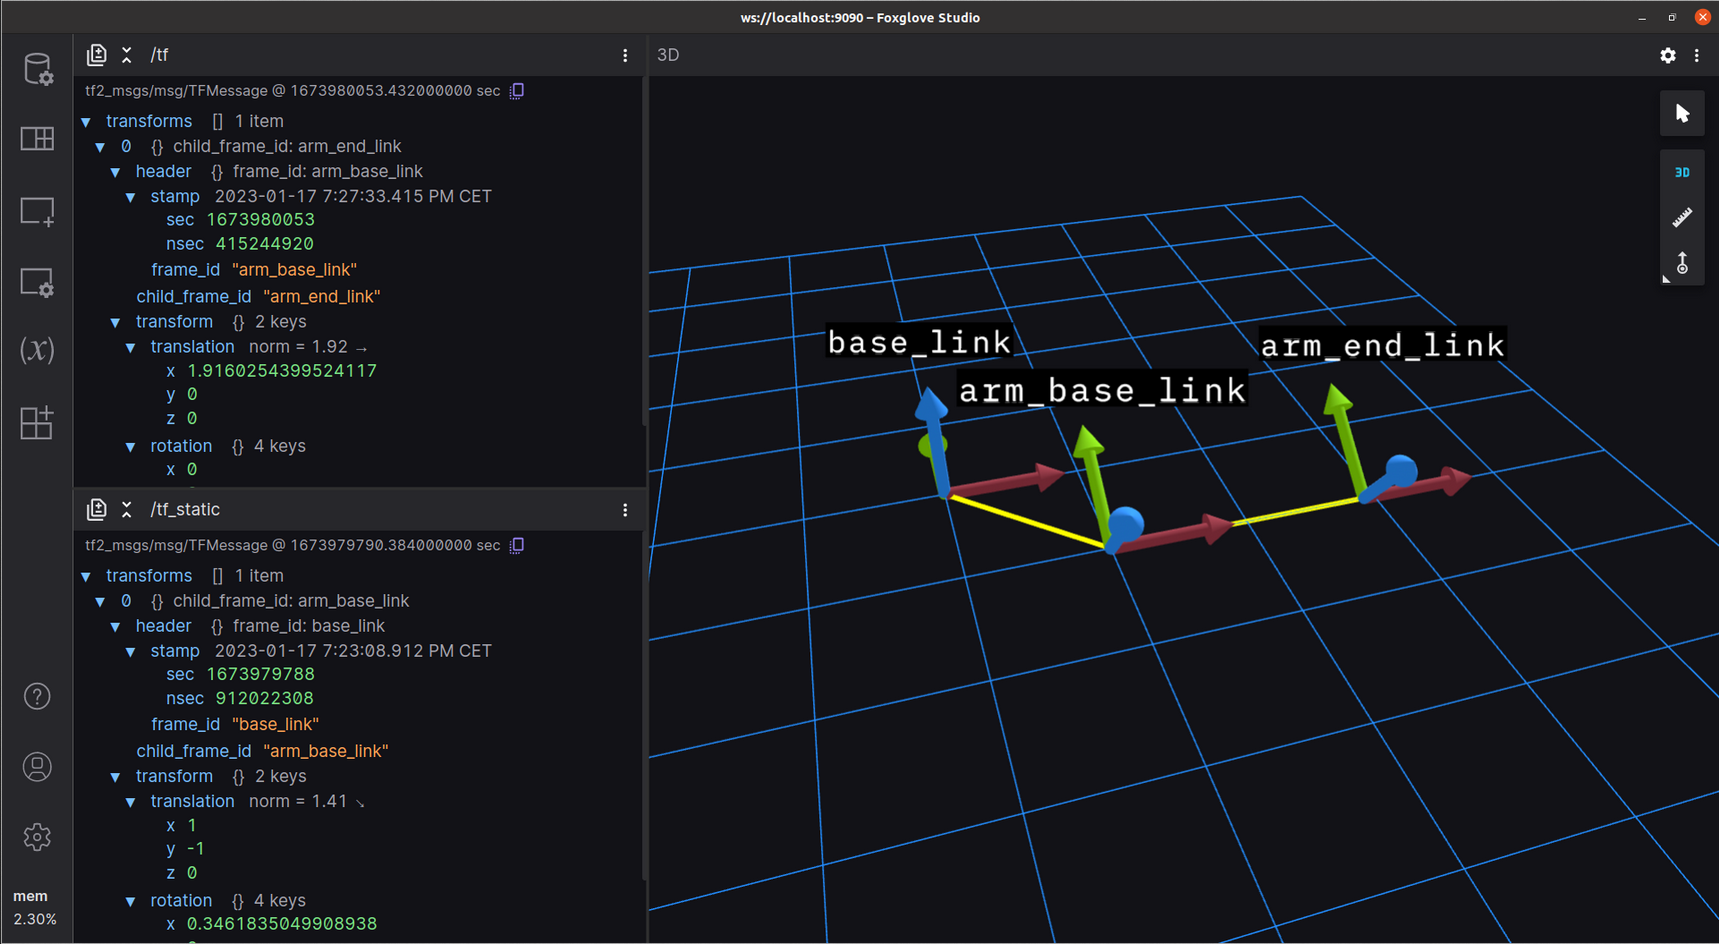
\includegraphics[width=\textwidth]{01_FoxgloveStudio.png}
            \caption{Visualizing ROS 2 Transforms with Foxglove Studio}
        \end{figure}

\section{State of WASM}

    \subsection{Unity in WebAssembly}

    % https://blog.unity.com/technology/webassembly-is-here
    % https://beta.unity3d.com/jonas/AngryBots/

    \begin{figure}[htbp]
        \centering
        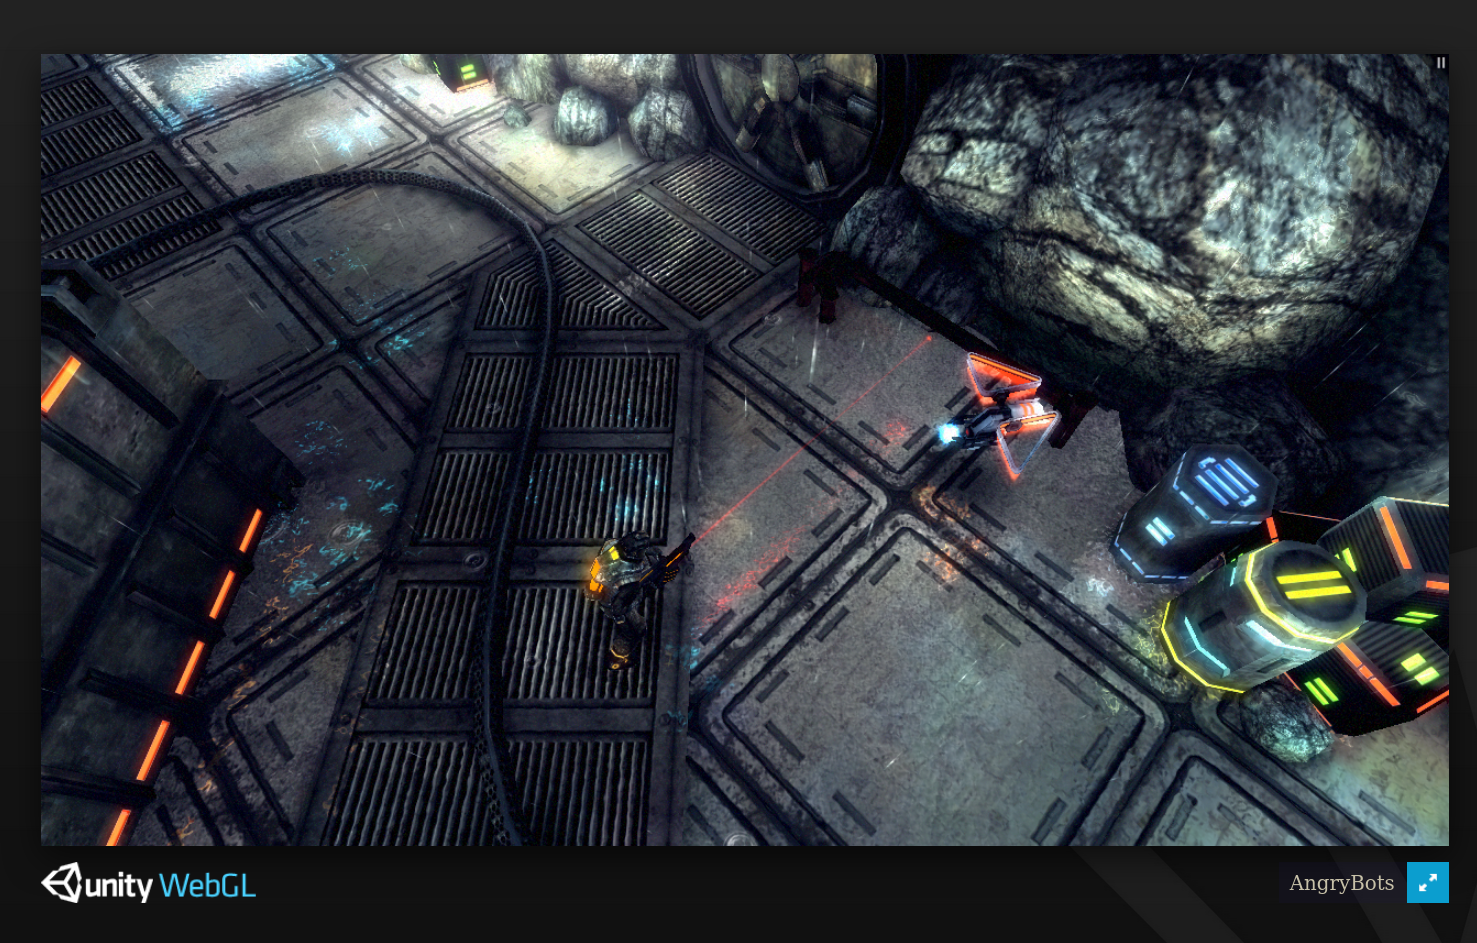
\includegraphics[width=0.8\textwidth]{01_angryBots.png}
        \caption{Demo of Angry Bots in Unity WebGL}\label{fig:unity}
    \end{figure}
